%!TEX root = Manuscrit.tex
\section{Apprentissage profond pour la vision artificielle}

\subsection{Historique de l'apprentissage profond}

La possibilité d'attribuer des capacités cognitives à un ordinateur a été originellement formalisé par Alan Turing en 1950~\cite{turing_computing_1950}. Turing propose un cadre formel permettant de répondre à la question \og{} une machine peut-elle penser \fg{} en définissant ce qui est désormais connu comme le test de Turing. Selon lui, un ordinateur intelligent serait défini par sa capacité à imiter un humain de manière à ce que d'autres individus soient incapables de discerner sa véritable nature. Toutefois, Turing ne répond pas à la question du \og comment \fg{} et ne propose pas d'implémentation permettant d'atteindre cet objectif.

Néanmoins, en 1943, Warren McCulloch et Walter Pitts proposaient un système de neurones booléens~\cite{mcculloch_logical_1943} munis de deux état\,: actifs ou inactifs. Ils définissent un neurone formel comme étant un automate fini muni d'une fonction de transfert, permettant de transformer un ensemble d'entrée en une valeur de sortie. Certains neurones ne recevaient aucun signal d'un autre neurone, mais formaient eux-mêmes l'ensemble du signal d'entrées pour le reste du réseau. Les autres neurones calculaient alors des combinaisons logiques à partir des signaux qu'ils recevaient en entrée. Les travaux de McCulloch et Pitts montrent que de nombreux prédicats de logique temporelle sont calculables par de tels réseaux booléens. Cette étude théorique est étendue par Kleene 1956 qui étudie notamment des réseaux booléens dont le graphe présente des cycles, c'est-à-dire des réseaux \emph{récurrents}. Kleene montre notamment que de tels réseaux sont capables de modéliser des langages rationnels, c'est-à-dire des langages définis par des expressions régulières~\cite{kleene_representation_1956}.

En parallèle, les travaux du neuropsychologue Donald Hebb sur les sciences cognitives ont permis de mettre en avant l'idée de l'apprentissage hebbien. Celui-ci explique le méchanisme d'apprentissage au sein du cerveau par le renforcement d'une connexion entre deux neurones à chacune de leurs activations simultanées~\cite{hebb_organization_1949}. Hebb théorise également la possibilité que des neurones se regroupent en \og{} assemblées de cellules \fg{} qui s'activeraient de façon synchronisée, formant ainsi une représentation mentale des signaux envoyés au cerveau. Comme nous allons le voir, ces deux idées forment une source considérable d'inspiration pour les méchanismes d'apprentissage en intelligence artificielle.

En 1957, Frank Rosenblatt définit le Perceptron~\cite{rosenblatt_perceptron:_1957}. Il s'agit d'un réseau de neurones acyclique, comme ceux de McCulloch et Pitts~\cite{mcculloch_logical_1943}. Les entrées et sorties sont booléennes et le réseau n'a qu'une seule couche. En outre, les poids des connexions sont déterminées automatiquement en utilisant la règle de Hebb~\cite{hebb_organization_1949}. Dans le cas où les données d'entrée sont linéairement séparables, le perceptron est assuré de pouvoir trouver la séparatrice optimale. Toutefois, le perceptron est un classifieur linéaire et ne peut donc pas résoudre de problèmes non-linéaires. Dans le livre \emph{Perceptrons}~\cite{minsky_perceptrons_1969}, Minsky et Papert montrent qu'un perceptron à une seule couche cachée est incapable de calculer la fonction XOR. Toutefois, il n'existe pas encore de bonne stratégie pour optimiser les poids d'un perceptron. Dans sa thèse soutenue en 1975~\cite{werbos_beyond_1975}, Paul Werbos formalise un algorithme de descente de gradient pour la minimisation d'erreur dans un réseau de neurones en utilisant le théorème de dérivation des fonctions composées, qu'il nomme \emph{backpropagation} (rétropropagation). Il faudra toutefois attendre dix ans pour voir apparaître les premières implémentations de l'algorithme de rétropropagation du gradient pour entraîner des perceptrons multi-couches~\cite{rumelhart_learning_1986,lecun_learning_1986}. Les neurones composant un perceptron multi-couches possèdent notamment une fonction de transfert non-linéaire, modélisant la réponse d'un neurone à une activation extérieure.

L'étude théorique des réseaux de neurones à propagation avant, et notamment des perceptrons, reprend alors. En 1989, George Cybenko démontre le théorème d'approximation universelle prouvant que les fonctions calculables par un perceptron sont denses dans l'ensembles des fonctions continues par morceaux, dans le cas de la sigmoïde comme fonction de transfert~\cite{cybenko_approximation_1989}. Ce résultat est étendu deux ans plus tard par Kurt Hornik en le généralisant à l'ensembles des fonctions d'activation~\cite{hornik_approximation_1991}. Le théorème formel est donné ci-dessous.

\begin{theorem}
Soit $\varphi$ une fonction bornée, croissante non-constante. Soit $C_0^n$ l'ensemble des fonctions continues définies sur $[0,1]^n$. Alors\,:
$$\forall \epsilon > 0, \forall f \in C_0^n, \exists N \in \mathbb{N}, \text{ des réels } v_i, b_i \in \mathbb{R} \text{ et des vecteurs } w_i \in \mathbb{R}^n \text{ avec } i \in \{1\dots{}n\} \text{ tels que}$$
$$F(x) = \sum_{i=1}^N v_i \varphi\left(w_i^t x + b_i \right)$$
soit une approximation de $f$ à $\epsilon$ près, c'est-à-dire\,:
$$\forall x \in [0,1]^n, ~\left| F(x) -f(x) \right| < \epsilon~.$$
\end{theorem}

En parallèle de ces avancées théoriques, les applications pratiques des perceptrons étaient étudiées, notamment dans le cadre de la vision artificielle pour la reconnaissance de formes. Ainsi, un des premiers problèmes étudiés est la reconnaissance de caractères écrits, en particulier les chiffres et les lettres. En 1980, Kunihiko Fukushima introduit le \emph{neocognitron}~\cite{fukushima_neocognitron:_1980}, un perceptron multi-couches dont la structure est inspirée par les travaux de Hubel et Wiesel sur les cortex visuels des chats et des singes~\cite{hubel_receptive_1959,hubel_receptive_1968}. Le neocognitron extrait des caractéristiques locales de l'image robustes aux légères déformations, qui sont graduellement combinées en cascade par le réseau. En 1989, Yann LeCun et collègues proposent une architecture de perceptron multi-couches dont la première couche est \emph{convolutive} pour la reconnaissance de chiffres manuscrits~\cite{lecun_backpropagation_1989}. Cette approche est reprise par la suite pour donner naissance à l'architecture LeNet-5~\cite{lecun_gradient-based_1998}, premier \gls{CNN} moderne. En 2004, les méthodes de détection et classification d'objets par \gls{CNN} sont évaluées comme étant compétitives, voire supérieure, que celles obtenues à partir de \gls{SVM} opérant directement sur les pixels. Des premiers travaux apparaissent utilisant les représentations apprises par les \gls{CNN} pour remplacer les descripteurs images \emph{ad hoc} comme \gls{SIFT}~\cite{lowe_object_1999} ou \gls{HOG}~\cite{dalal_histograms_2005} pour la classification d'objets~\cite{serre_object_2005,huang_large-scale_2006}.

En 2006, Hinton et Salakhutdinov introduisent les réseaux de neurones auto-encodeurs pour la réduction de dimension~\cite{hinton_reducing_2006}. Leur approche utilise une pile de machines de Boltzmann restreintes~\cite{ackley_learning_1985,salakhutdinov_deep_2009}, entraînées successivement couche par couche, chacune étant traitée comme entrée pour la suivante. Ce modèle hybride exploré dans un article de 2006~\cite{hinton_fast_2006} qui leur donne le nom de \gls{DBN}. L'année suivante, une équipe menée par Yoshua Bengio étend ce pré-entraînement par couche à des \gls{DBN} pour la régression. En outre, leurs travaux suggèrent que le pré-entraînement permet d'initialiser les couches supérieures à partir de meilleures représentations des abstractions de haut niveau que l'initialisation aléatoire~\cite{bengio_greedy_2007}. Bengio défend par ailleurs l'idée qu'un bon algorithme d'apprentissage doit être capable, en temps raisonnable, d'apprendre des représentations sémantiques pertinentes à des niveaux d'abstraction variés à partir de données non nécessairement annotées, c'est-à-dire en apprentissage non supervisé. Il argumente en faveur des modèles profonds comme étant plus expressives et pouvant apprendre des meilleures représentations~\cite{bengio_learning_2009} en s'appuyant sur des travaux en neurosciences concernant le cortex visuel~\cite{serre_quantitative_2007}.

Par ailleurs, c'est également en 2006 que les premières implémentations des \gls{CNN} sur \gls{GPU} voient le jour~\cite{chellapilla_high_2006} pour le traitement automatisée de documents. En 2011, Dan Cire\c{s}an proposent des méthodes à base de \gls{CNN} qui obtiennent la première place dans deux compétitions\,: reconnaissance de caractères chinois~\cite{liu_icdar_2011} et classification de panneaux de signalisation~\cite{stallkamp_german_2011}. En 2010, la compétition \gls{ILSVRC} de reconnaissance d'objets démarre en utilisant la banque de données ImageNet~\cite{deng_imagenet:_2009} comme référence. Un million d'images sont annotées pour mille classes d'intérêt différentes. En 2012, la compétition est remportée par Alex Krizhevsky, Ilya Sutskever et Geoffrey Hinton à l'aide du réseau convolutif profond AlexNet~\cite{krizhevsky_imagenet_2012} implémenté sur \gls{GPU} à l'aide de la bibliothèque \gls{CUDA}. AlexNet obtient 15\% d'erreur, tandis que la seconde méthode du podium n'obtient que 26\%. Ce succès a été à l'origine de l'explosion en popularité des réseaux convolutifs et de l'apprentissage profond, notamment dans la communauté vision. La compétition \gls{ILSVRC} est depuis dominée par les approches \gls{CNN}, aussi bien en reconnaissance qu'en détection et segmentation d'objets. Le succès récent des réseaux convolutifs profonds est donc dû à la convergence de trois facteurs\,: des avancée théoriques (\gls{ReLU}, réceaux convolutifs) permettant d'entraîner des réseaux plus profonds, la mise à disposition de grandes bases de données annotées pour l'apprentissage supervisées et des implémentations rapides sur \gls{GPU} rendant les temps de calcul tolérables.

\subsection{Réseaux de neurones artificiels}

\begin{figure}
  \resizebox{\textwidth}{!}{
  \documentclass{standalone}
\usepackage[utf8]{inputenc}
\usepackage[T1]{fontenc}
\usepackage{tikz}
\begin{document}
  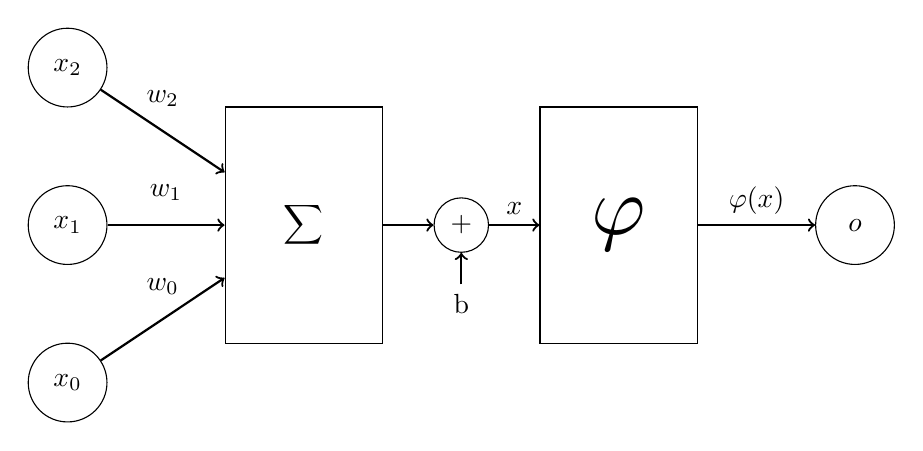
\begin{tikzpicture}

  \node[rectangle, draw=black, minimum size=2cm,minimum height=3cm] (sum) at (3, 0) {$\displaystyle\sum$};

  \foreach\name in {0,1,2}{
      \pgfmathsetmacro\y{2*\name-2}
  	\node[circle, draw=black,minimum size=1cm] (input\name) at (0, \y) {$x_{\name}$};
      \draw[thick,->] (input\name) to node[yshift=5pt,above] {$w_{\name}$} (sum);
  }

  \node[rectangle, draw=black, minimum size=2cm,minimum height=3cm] (phi) at (7, 0) {};
  \node[scale=3] (phisym) at (phi.center) {$\displaystyle\varphi$};

  \node (bias) at (5, -1) {b};
  \node[circle, draw=black] (sumb) at (5, 0) {$+$};
  \draw[thick,->] (sum.east) -- (sumb.west);
  \draw[thick,->] (bias.north) -- (sumb.south);
  \draw[thick,->] (sumb.east) -- node[above] {$x$} (phi.west);
  \node[circle,draw=black,minimum size=1cm] (out) at (10,0) {$o$};
  \draw[thick,->] (phi.east) -- node[above] {$\varphi(x)$} (out.west);
  \end{tikzpicture}
\end{document}


  }
\caption{Modélisation d'un neurone artificiel.}
\label{fig:neurone}
\end{figure}

\begin{figure}
  \begin{subfigure}[b]{0.5\textwidth}
    \includegraphics[width=\textwidth]{activations}
    \caption{Fonctions d'activation saturantes.}
    \label{fig:activations}
  \end{subfigure}
\begin{subfigure}[b]{0.5\textwidth}
  \includegraphics[width=\textwidth]{rectifiers}
  \caption{Fonctions d'activation non-saturantes.}
  \label{fig:rectifiers}
\end{subfigure}
\caption{Exemples de fonctions d'activation.}
\label{fig:activations}
\end{figure}

\begin{figure}
  \begin{subfigure}[b]{0.5\textwidth}
    \resizebox{\textwidth}{!}{
    \documentclass{standalone}
\usepackage[utf8]{inputenc}
\usepackage[T1]{fontenc}
\usepackage{tikz}
\input{../CommandesPerso.tex}
\begin{document}
  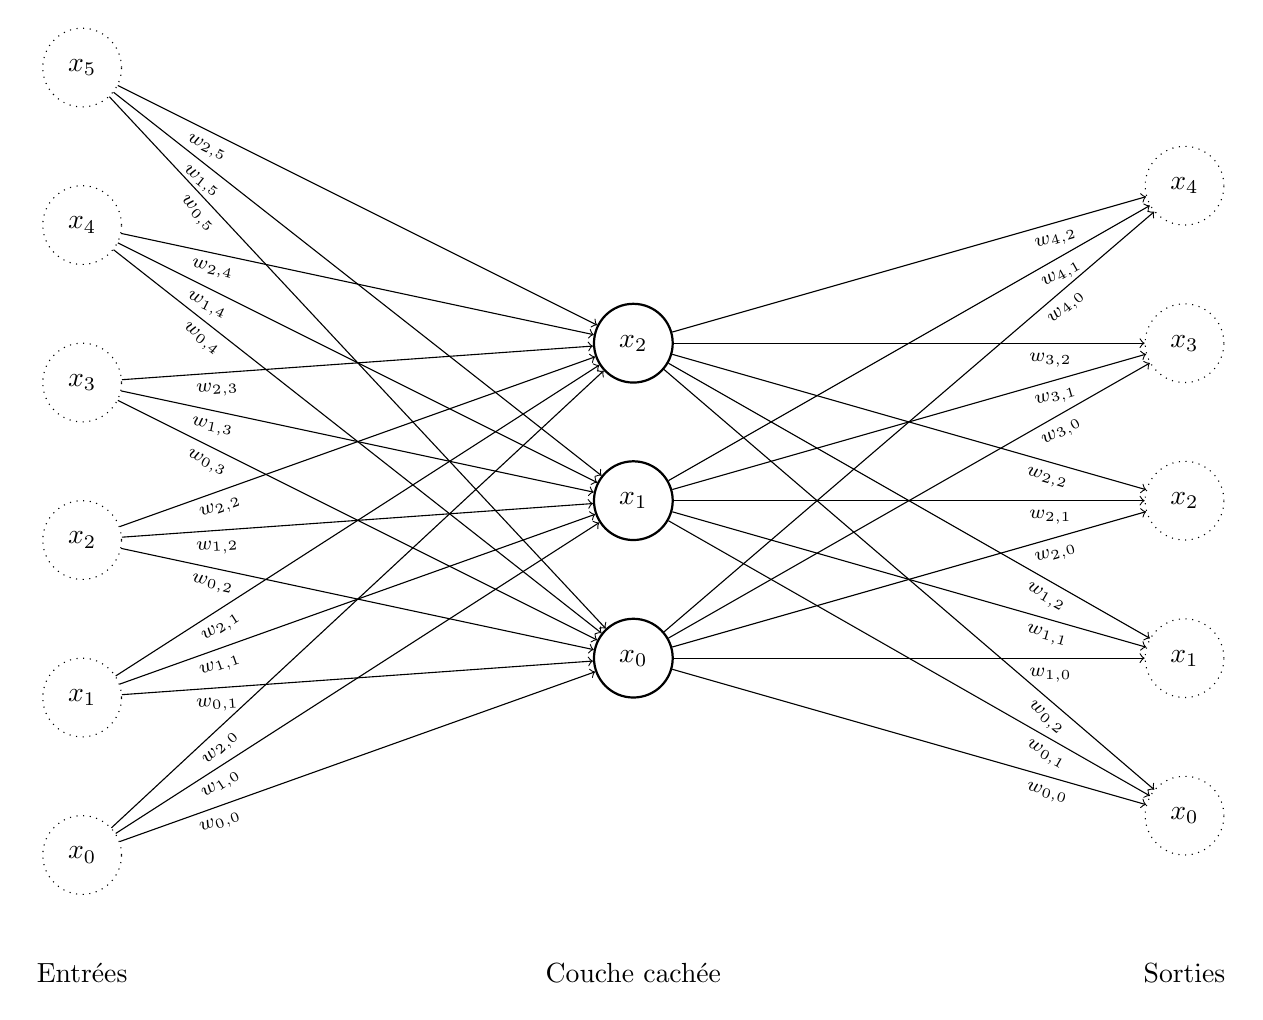
\begin{tikzpicture}
  \foreach\name in {0,1,2,3,4}{
      \pgfmathsetmacro\y{2*\name-3}
  	\node[circle, dotted,draw=black,minimum size=1cm] (output\name) at (7, \y) {$x_{\name}$};
  %    \draw[thick,->] (input\name) to node[yshift=5pt,above] {$w_{\name}$} (sum);
  }

  \foreach\name in {0,1,2}{
      \pgfmathsetmacro\y{2*\name-1}
  	\node[circle, thick,draw=black,minimum size=1cm] (hidden\name) at (0, \y) {$x_{\name}$};
      \foreach\oname in {0,1,2,3,4}{
      \draw[->] (hidden\name) to node[near end, sloped,pos=0.8,below] {\scriptsize $w_{\oname,\name}$} (output\oname);
      }
  }

  \node at (-7, -5) {Entrées};
  \node at (0, -5) {Couche cachée};
  \node at (7, -5) {Sorties};

  \foreach\name in {0,1,2,3,4,5}{
      \pgfmathsetmacro\y{2*\name-3.5}
  	\node[circle, dotted, draw=black,minimum size=1cm] (input\name) at (-7, \y) {$x_{\name}$};
      \foreach\hname in {0,1,2}{
      \draw[->] (input\name) to node[near end, sloped,pos=0.2,below] {\scriptsize $w_{\hname,\name}$} (hidden\hname);
      }
  }
  \end{tikzpicture}
\end{document}

    }
  \caption{Perceptron à une couche cachée.}
  \end{subfigure}%
  \begin{subfigure}[b]{0.5\textwidth}
    \resizebox{\textwidth}{!}{
    \documentclass{standalone}
\usepackage[utf8]{inputenc}
\usepackage[T1]{fontenc}
\usepackage{tikz}
\usepackage{ifthen}
\input{../CommandesPerso.tex}
\begin{document}

    \begin{tikzpicture}

    \newcommand\drawlayer[7]{%{nombre de neurones}{position en x}{symbole}{nom de la couche}{couche précédente}{n couche précédente}{style}
      \foreach\name in {0,...,#1}{
        \pgfmathsetmacro\y{2*(\name-#1/2)}
      	\node[circle,#7,draw=black,minimum size=1cm] (#4_\name) at (#2, \y) {$#3_{\name}$};
          \ifthenelse{\equal{#5}{}}{}{
		\foreach\oname in {0,...,#6}{
	            {\draw[->] (#5_\oname) to (#4_\name);}
         	 }
      	  }
      }
    }

    \drawlayer{5}{0}{x}{input}{}{}{dotted}
    \drawlayer{3}{4}{h^1}{hidden1}{input}{5}{thick}
    \drawlayer{4}{8}{h^2}{hidden2}{hidden1}{3}{thick}
    \drawlayer{3}{12}{h^3}{hidden3}{hidden2}{4}{thick}
    \drawlayer{3}{16}{y}{output}{hidden3}{3}{dotted}

    \node at (0,-6.5) {Entrées};
    \node at (8,-6.5) {Couches cachées};
    \node at (16,-6.5) {Sorties};

    \end{tikzpicture}

\end{document}


    }
  \caption{Perceptron multi-couches.}
  \end{subfigure}
  \caption{Perceptron à une et plusieurs couches. Les entrées et sorties peuvent être de dimensions variables et sont représentées comme des neurones.}
  \label{fig:perceptron}
\end{figure}

La définition formelle d'un neurone artificiel a été introduite par McCulloch et Pitts~\cite{lettvin_what_1959} en 1959. Un neurone doté d'une fonction de transfert $\varphi$ opère sur un ensemble de $n$ neurones d'entrée émettant chacun une valeur $x_1\dots{}x_n$, auxquelles il est connecté par des synapses de poids $w_i$. La valeur d'entrée $x$ du neurone correspond à la somme pondérée des signaux d'entrée. Le neurone émet ensuite l'image $o = \varphi(x)$ de ce signal par sa fonction de transfert. Le schéma de la~\cref{fig:neurone_schema} décrit ce procédé. L'activation en sortie d'un neurone s'obtient donc par la formule
$$o = \varphi\left(\sum_{i=1}^n w_i x_i + b\right)~.$$

Plusieurs neurones connectés les uns aux autres forment un graphe orienté et pondéré. Un réseau de neurones à propagation avant désigne un graphe neuronal acyclique. En pratique, on considère des graphes multipartis que l'on peut alors représenter par \fg couches \og{}. Dans le cas d'un perceptron à couches multiples, les valeurs du signal d'entrée sont placées dans une couche d'entrée et les signaux de sortie envoyés dans une couche de sortie. La ou les couches de neurones réellement optimisables sont nommées \og couches cachées \fg{} et font l'interface entre l'entrée et la sortie. Le perceptron multi-couches à une et plusieurs couches cachées sont illustrés dans la~\cref{fig:perceptron}.

La fonction d'activation des neurones peut prendre de nombreuses formes. Il est \emph{a minima} nécessaire que celle-ci soit non-linéaire, sans quoi elle rend le perceptron multi-couches équivalent au perceptron simple, et presque partout différentiable afin de pouvoir appliquer l'algorithme de rétropropagation du gradient. La fonction d'activation est en outre généralement choisie monotone croissante et de dérivée monotone croissante. La~\cref{fig:activations} illustre plusieurs activations communément utilisées dans les réseaux de neurones artificiels profonds\,:
\begin{itemize}
  \item La \textbf{sigmoïde}, ou fonction logistique\,: $\sigma(x) = \frac{1}{1 + e^{-x}}$.
  \item La fonction \textbf{tangente hyperbolique}\,: $\tanh(x) = \frac{1 - e^{-2x}}{1 + e^{-2x}}$.
  \item La \textbf{marche de Heavyside}\,: $H(x) = 0 \text{ si } x < 0 \text{ et } 1 \text{ si } x \geq 0$.
  \item La fonction \textbf{\gls{ReLU}}\,: $ReLU(x) = max(0,x)$.
  \item La fonction \textbf{SoftPlus}\,: $s(x) = ln(1 + e^x)$.
\end{itemize}

La fonction sigmoïde, bien que populaire à l'origine, est une fonction saturante qui souffre de gradients évanescents. Ce problème n'est pas circonscrit à la sigmoïde et est particulièrement pregnant dans le cas des réseaux de neurones récurrents~\cite{hochreiter_gradient_2001}. L'accumulation de couches dans un réseau fait que la rétropropagation du gradient est similaire à une suite géométrique. Le produit cumulé de $n$ gradients dans des fonctions d'activation à tendance contractante produit un $n+1$ gradient plus faible que le précédent, et ainsi de suite. À l'inverse, il est possible d'avoir des gradients explosifs. Ce problème est empiré dans le cas des fonctions saturants comme la sigmoïde ou la tangente hyperbolique car leurs gradients sont nécessairement dans $[0,1]$. L'utilisation de la sigmoïde ou la tangente hyperbolique a varié dans la littérature. LeCun~\cite{lecun_efficient_1998} recommande d'utiliser la fonction hyperbolique modifiée $f(x) = 1,7159 tanh(\frac{2}{3} x)$, notamment car celle-ci est bornée par $[-1,1]$ et centrée en 0, ce qui est adapté au travail sur des données normalisées à moyenne nulle et variance unitaire.

La marche de Heavyside, tout comme la fonction $signe$, a des gradients nuls presque partout, sa dérivée étant l'impulsion de Dirac $\delta$.

Pour limiter les gradients évanescents, des fonctions non-linéaires non-saturantes sont désormais majoritairement utilisées dans la littérature. Glorot, Bordes et Bengio~\cite{glorot_deep_2011} ont ainsi proposé d'utiliser la fonction \gls{ReLU}, introduite précédemment pour les \gls{DBN}~\cite{nair_rectified_2010}, et la fonction SoftPlus pour les réseaux de neurones artificiels de toutes sortes. Leurs travaux aboutissent à trois conclusions importantes. Tout d'abord, les fonctions d'activation non-linéaire obtiennent généralement de meilleures performances que les réseaux utilisant $tanh$. Ensuite, les réseaux entraînés avec \gls{ReLU} ne nécessitent pas de pré-apprentissage non-supervisé couche par couche, ce qui accélère grandement les temps d'entraînement. Enfin, ces modèles sont plus parcimonieux que leurs équivalents usuels. En outre, la fonction \gls{ReLU} est simple à implémenter et rapide à calculer, ce qui a contribué à sa popularisation rapide dans la communauté.

Plusieurs variantes ont dès lors été proposées autour des fonctions linéaires rectifiées, notamment une version paramétrique dont la partie négative est non-saturante, mais linéaire de pente $\alpha$ fixée par l'utilisateur (\emph{Leaky ReLU}~\cite{maas_rectifier_2013}) ou optimisable (\gls{PReLU}~\cite{he_delving_2015}). Une version similaire mais continue a également été proposée sous la forme des \gls{ELU}~\cite{clevert_fast_2015}. Plus récemment, une recherche automatique quasi-exhaustive sur une variété de fonctions d'activation possibles a permis de proposer la \emph{Swish}~\cite{ramachandran_searching_2018}, non-linéaire non-saturante mais ayant la particularité d'être non-monotone. Ces variantes sont illustrées dans la~\cref{fig:rectifiers} et leur formule est donnée ci-dessous\,:
\begin{itemize}
  \item La fonction \textbf{\emph{Leaky ReLU}}\,: $LReLU_\alpha(x) = max(0,x) - \alpha max(0,-x)$, avec $\alpha$ un hyperparamètre.
  \item La fonction \textbf{\gls{PReLU}}\,: $PReLU(x, \alpha) = max(0,x) - \alpha max(0,-x)$, avec $\alpha$ optimisable.
  \item La fonction \textbf{\gls{ELU}}\,: $ELU_\alpha(x) = x \text{ si } x > 0 \text{ et } \alpha (exp(x) - 1) \text{ sinon}$.
  \item La fonction \textbf{\emph{Swish}}\,: $Swish_\beta(x) = x . \sigma(\beta x) = x . (1 + e^{-\beta x})^{-1}$.
\end{itemize}
% TODO : ref Oyallon sur les "bonnes" hypothèses pour la fonction d'activation

Le théorème d'approximation universelle~\cite{cybenko_approximation_1989,hornik_approximation_1991} indique que l'ensemble des fonctions engendrées par les perceptrons est dense dans l'ensemble des fonctions continues par morceaux sur des compacts. Autrement dit, toute fonction $f : E \rightarrow \mathbb{R}^m$ avec $E = \bigcup\limits_{k} C_k$ une union de compacts de $\mathbb{R}^n$ continue sur chaque compact est approximable à une précision $\epsilon$ arbitraire par un perceptron. On peut voir deux limitations à ce résultat. Le premier concerne la nature de la fonction d'activation. Le théorème généralisé par Hornik s'applique à tous les perceptrons sur lesquels on applique une fonction d'activation monotone non-constante et bornée, cela couvre les fonctions saturantes $tanh$ et sigmoide, mais exclut les fonctions linéaires rectifiées comme \gls{ReLU}. Ce problème a cependant été levé par Sonoda et Murata~\cite{sonoda_neural_2017}, qui ont montré que des réseaux munis de fonctions d'activation non-bornées satisfaient tout de même le théorème d'approximation universelle


La deuxième limitation porte quant à elle sur la nature même du théorème. Celui-ci ne donne qu'une garantie purement théorique concernant l'existence d'un ensemble de paramètres permettant l'approximation à la précision voulue. Il ne donne pas de bornes sur le nombre de neurones nécessaire, ni de méthode de construction. Ainsi, il n'y aucune certitude que les poids puissent être obtenus par descente de gradient, ni d'indication sur l'architecture à choisir. En particulier, le théorème vaut pour des réseaux superficiels à une seule couche. Pourtant, le consensus scientifique dans la communauté tend à préférer des réseaux de plus en plus profonds. Ainsi, il a été démontré que des réseaux plus profonds demandent moins de poids et de neurones pour approximer des fonctions plus complexes~\cite{bianchini_complexity_2014,mhaskar_when_2017}. En particulier, la structure hiérarchique des réseaux multi-couches semble adapté à l'approximation de fonctions composées en contournant la malédiction de la dimension~\cite{poggio_why_2017}. Toutefois, cela augmente également le nombre d'hyperparamètres à régler pour définir l'architecture. L'absence de méthode systématique de construction des architectures de réseau profond conduit donc à l'utilisation intensive de la méthode essai-erreur ou à des méthodes de méta-apprentissage~\cite{zoph_neural_2016}.

\subsection{Réseaux de neurones convolutifs profonds}

Briques de base\,: opérateur de convolution, opérateur de sous-échantillonnage.

L'idée de partager des poids pour réaliser de façon dense la même opération locale sur toute l'image remonte au Neocognitron~\cite{fukushima_neocognitron:_1980}. L'idée d'utiliser des convolutions remonte à LeCun~\cite{lecun_gradient-based_1998}.

Les convolutions avaient déjà été utilisées de nombreuses fois. Notamment, les Gabor, les HOG, les SIFT et les ondelettes ! Mais ici on se propose de mettre des noyaux de convolution optimisables. L'apprentissage par représentation va donc se faire naturellement dans le domaine image avec des opérateurs adaptés.

\subsection{Entraînement des réseaux de neurones}

Un autre inconvénient au théorème d'approximation universelle est que même si l'architecture était connue, celui-ci ne donne aucune méthode pour trouver les valeurs des paramètres. En particulier, l'algorithme de rétropropagation du gradient~\cite{werbos_beyond_1975,rumelhart_learning_1986,lecun_learning_1986} décrit ci-après se base sur une méthode de descente de gradient. Toutefois, rien ne garantit que les poids optimaux dont l'existence est assurée par le théorème d'approximation universelle ne soit trouvables par cet algorithme.

L'algorithme de rétropropagation du gradient se fonde sur la règle de dérivation en chaîne, c'est-à-dire le théorème de dérivation des fonctions composées~\cite{lhospital_analyse_1716,lagrange_theorie_1797}\,:
\begin{theorem}
Soient $f$ et $g$ deux fonctions telles que $f : I \rightarrow J \subset \mathbb{R}$ et $g : J \rightarrow \mathbb{R}$. Soit $x \in I$ tel que $f$ admet une dérivée en $x$. Alors, la fonction composée $h = g \circ f : I \rightarrow \mathbb{R}$ admet une dérivée en $x$ de valeur :
$$h'(x) = (g \circ f)'(x) = f'(x) \times g'(f(x))~.$$

Si $f$ et $g$ sont dérivables respectivement sur $I$ et $J$, alors\,:
$$(g \circ f)' = f' \times (g' \circ f)~.$$

ou encore, en utilisant la notation de Leibniz, avec $z = g(y)$ et $y = f(x)$:
$$\frac{dz}{dx} = \frac{dz}{dy} \times \frac{dy}{dx}~.$$
\end{theorem}

Ce théorème s'étend aux dérivées partielles de fonctions à valeurs dans $\mathbb{R}^n$.

Dans le cas des réseaux profondes, la propagation avant des activations se fait par la formule suivante\,:
$$z_j^{k+1} = \varphi\left(\sum_{i=1}^n w^k_{i,j} \cdot z^k_i + b^k_j\right)$$
avec $\varphi$ la fonction d'activation, $w_{i,j}$ le poids de la connexion, $b_i$ le biais et $k$ le numéro de la couche.

En connaissant l'erreur $e^{k+1}$, c'est-à-dire le gradient pour la couche $k+1$, alors\,:

$$e^k_j = \sum_{i=1}^N w^k_{i,j} e^{k+1}_j  \varphi'\left(\sum_{i=1}^n w^k_{i,j} \cdot z^k_i + b^k_j\right)$$

Pour diminuer l'erreur, il est nécessaire de mettre à jour les poids $w^k$ dans la direction opposée au gradient $\frac{de}{dw^k}$. Or, grâce à la règle de la dérivation en chaîne\,:
$$\frac{de}{dw^k} = \frac{de}{dz^k} \times \frac{dz^k}{dw^k}$$.

Il est donc possible de calculer la mise à jour des poids en rétro-propageant la valeur du gradient d'une couche à la précédente.

On peut alors utiliser l'algorithme de descente de gradient~\cite{cauchy_comptes_1847} afin de minimiser l'erreur totale en mettant à jour les poids.

L'algorithme utilisé pour être soit l'algorithme exact, qui calcule l'erreur sur l'ensemble du jeu de données et obtient la direction exacte du gradient permetant de minimiser l'erreur, soit l'algorithme stochastique, qui estime en ligne le gradient à partir d'un échantillon unique, soit l'algorithme stochastique par \emph{mini-batch}, qui estime à partir d'un ensemble de données le gradient. % TODO : détailler
% TODO: variantes de la SGD

% TODO: tips and tricks sur la SGD (Bottou, LeCun, Bengio)
Il est important de noter que la descente de gradient minimise l'erreur sur le jeu d'entraînement, tandis que l'erreur qui nous intéresse réellement est celle de généralisation. Toutefois, nous n'avons pas accès à cette erreur et devons donc nous contenter de celle disponible.

% TODO : détailler
Régularisation (dropout, pénalité sur les poids, initiliasitation pour contourner les problèmes dûs à la descente de gradient)

% TODO : détailler
Fonctions de coût : régression\,: L1, L2 (et variantes "Huber"), classification\,: cross-entropy

\subsection{Réseaux de neurones et apprentissage multi-modal}

L'apprentissage multi-modal via des réseaux de neurones se raccorde au problème d'apprentissage de représentation incluant plusieurs sens. ~\cite{baltrusaitis_multimodal_2017} propose la taxonomie suivante, dans laquelle les représentations peuvent être conjointes (une même représentation pour plusieurs modalités) ou coordonnées (chaque modalité à une représentation)\,:
\begin{itemize}
    \item Traduction\,: convertir d'une modalité à une autre.
    \item Alignement\,: trouver des correspondances (au sens bijectif) entre une représentation d'une modalité et une autre.
    \item Fusion\,: l'intégration de plusieurs modalités dans la prise de décision.
    \item Apprentissage conjoint\,: apprendre une représentation à partir des différentes modalités.
\end{itemize}

Les travaux en fusion de données sont anciens. On peut citer la fusion amont ou la fusion aval ("tardive"), qui peut être approchée par la notion de moyenne pondérée, proche dans l'idée des ensembles de modèles. C'est ainsi l'approche traditionnelle utilisée en 1989 pour la fusion audio-image~\cite{yuhas_integration_1989}.

Approche de fusion avec des HMM pour l'audio-vidéo~\cite{noda_audio-visual_2015}.

Approche d'apprentissage sur représentation conjointe en audio-image~\cite{ngiam_multimodal_2011} et audio-texte~\cite{srivastava_multimodal_2014}. Récemment,~\cite{eitel_multimodal_2015} propose une fusion tardive où la dernière couche apprend une représentation conjointe, même chose en audio-image pour~\cite{mroueh_deep_2015}. % TODO: note pour moi-même: Hazirbas fait la même chose mais il joint les représentations intermédiaires. Nous, on fait quelque chose de proche d'Eitel mais plutôt dans une idée de chercher la représentation de ce qui est discriminant chez chaque modalité.

Datasets :
texte + image~\cite{hodosh_framing_2013}
diverses acquisitions de MR scan~\cite{menze_multimodal_2015}
3D + image + senseurs~\cite{ofli_berkeley_2013}
aduio + video + ECG + EDGA pour les émotions~\cite{ringeval_introducing_2013}
audio + video pour les émotions~\cite{schuller_avec_2011}

\section{Apprentissage profond pour la segmentation sémantique}

\subsection{Segmentation sémantique et classification}

La classification d'images dans des challenges comme ImageNet~\cite{russakovsky_imagenet_2015} ou des jeux de données CIFAR-10 et CIFAR-100~\cite{krizhevsky_learning_2009} permet d'effectuer de la reconnaissance d'objet. Toutefois, cela ne donne pas d'information directement concernant leur localisation. Certains se sont intéressés à la détection d'objet.

Des progrès considérables ont été réalisés depuis le succès d'AlexNet~\cite{krizhevsky_imagenet_2012}, notamment\,:
les modèles VGG~\cite{chatfield_return_2014} et \cite{simonyan_very_2014}
le modèle Inception~\cite{szegedy_going_2015} et ses variantes~\cite{szegedy_rethinking_2015,szegedy_inception-v4_2016}
Le modèle ResNet~\cite{he_deep_2016}
Puis le modèle DenseNet~\cite{huang_densely_2017}

Mais en réalité on veut surtout faire de la segmentation sémantique, avec dans l'idée la compréhension de scène. Plusieurs jeux de données existent pour des images multimédia classiques~\cite{everingham_pascal_2014,lin_microsoft_2014} ou avec un focus sur la conduite autonome~\cite{cordts_cityscapes_2016,neuhold_mapillary_2017}.

On peut commencer par faire de la localisation à partir de features denses sur l'image.


\subsection{Approches entièrement convolutives}

\cite{long_fully_2015}
Amélioration par ~\cite{l._c._chen_deeplab_2018} et~\cite{yu_multi-scale_2015} avec la convolution à trous pour étendre le FoV
Utilisation des CRF ad nauseam~\cite{arnab_higher_2015,zheng_conditional_2015}
Approches "à la encodeur"~\cite{zhao_stacked_2015-1} avec SegNet~\cite{badrinarayanan_segnet_2017} et DeconvNet~\cite{noh_learning_2015} et U-Net~\cite{ronneberger_u-net_2015}
Bidules et machins multi-échelles et globaux~\cite{nekrasov_global_2016}
Passage au ResNet~\cite{wu_high-performance_2016} et DenseNet~\cite{jegou_one_2017}

\section{Apprentissage pour le traitement d'images de télédétection}

\subsection{Différents types d'imagerie}

\subsection{Classification d'images de télédétection}
UC-Merced, Brazilian Coffe

Approches par patch

\subsection{Segmentation sémantique d'images de télédétection}
ISPRS, Inria, DFC
En hyperspectral


\bibliographystyle{acm}
\bibliography{Chapitre1/Historique}
